\section{Les classes \enquote{agents}}
\subsubsection{Sprints 1 et 2}
Lors du premier sprint, nous avons commencé par mettre en place la base du programme. Nous avions prévu de faire l'UML~\ref{v0.1}.

 Pour le modèle, il s'agissait de créer les classes :
\begin{itemize}
\item Turtle, qui représente une tortue~;
\item Point, pour stocker les coordonnées d'une tortue~;
\item Line, qui est composé de points, et qui permet aux tortues de laisser une trace (instruction \verb|pen_down|)~;
\item World.
\end{itemize}


\begin{figure}[h]
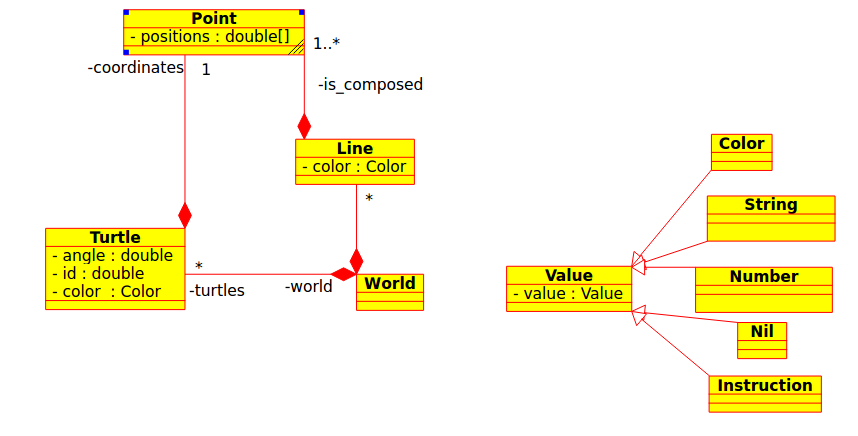
\includegraphics[scale=0.5]{doc/report/uml/v01.png}
\caption{\label{v0.1} UML prévisionnel de la version 0.1}
\end{figure}


La classe World représente le monde. Il contient la liste des tortues, et les lignes tracées par celles-ci car c'est lui qui communique avec l'interface pour l'affichage de ces lignes.
À la fin du sprint 1, on pouvait voir une tortue avancer et tracer une ligne sur son passage.
Nous avions réalisé le schéma \ref{v0.1R}. Il respecte la version prévue, en dehors de la classe Instruction, qui n'était finalement pas nécessaire, les instructions étant des mot-clés du langage.

Lors du second sprint, nous avons ajouté une classe Agent, super classe de World, Turtle et Zone. En effet, elles sont toutes les trois des agents, et ont donc des comportements similaires (cf. Figure~\ref{v0.2}).

Ces classes ont chacun un parent, représentant l'agent qui l'a créé, une liste d'enfants, et des propriétés. Les propriétés sont des variables définit par l'utilisateur lors de la définition du code de l'agent, donc surtout utile pour les tortues.

De plus, le monde a une taille et deux listes d'espèce de tortues (dit «~breed~»)~: les espèces nommées et les anonymes, qui sont des «~turtles~» dans le code.

Comme le montre le listing \ref{nameTurtle}, on peut créer des tortues nommées ou pas. Une tortue anonyme a son corps défini à la création de l'agent (lors du \verb|new agent|) tandis que les tortues nommées on leur corps défini lors de la création du «~breed~» (instruction \verb|agent <nom>|).

\begin{lstlisting}[label=nameTurtle,caption=Nommage lors de la création d'une tortue]
agent listener () {
	fd 2
}

new listener ()

new agent {
	lt 30
	fd 5
}
\end{lstlisting}

\subsubsection{Sprints 3 et 4}
Lors du troisième sprint, nous avons mis en place des pointers intelligents dans toutes nos classes (cf. Figure~\ref{v0.3}). Le but de ce sprint était la mise en place de la communication entre les agents~: les tortues devaient pouvoir communiquer avec les zones par écriture dans leurs propriétés, et elles devaient aussi pouvoir communiquer entre elles grâce à des instructions comme \verb|send| et \verb|recv|.

L'étape suivante était d'ajouter des fonctionnalités tel que la maîtrise du temps et l'exportation du modèle. Ces ajouts ne provoquent pas de changement du coté du modèle, si ce n'est quelques méthodes dans les classes World, Turtle et Zone pour l'exportation du modèle.
Celle-ci consiste à créer une sauvegarde de l'état du modèle à un instant \verb|t| dans un fichier JSON grâce à la bibliothèque JSON Spirit.
Cela permettra ensuite, par exemple en passant par une transformation en CSV, d'avoir des tableaux avec toutes les données, ce qui offre la possibilité d'avoir des diagrammes de l'évolution du monde.

La maîtrise du temps se fait grâce à un bouton pause, qui arrête les threads s'exécutant, ou par un slider qui permet de ralentir ou de diminuer la vitesse.

\section{Les types}
\subsubsection{Sprints 1 et 2}
Lors du premier sprint, nous avons mis en place un certains nombre de types, comme \verb|Color|, pour la couleur, ou encore \verb|Nil| qui a une valeur nulle. Ils héritent de \verb|Value|, une classe abstraite qui contient une valeur et ses accesseurs.
%Les instructions tel que pen\_down, forward, etc., sont finalement des mots clés dans la grammaire du langage, et non pas des méthodes de la classe Instructions, contrairement à ce que nous avions prévu (cf. UML~\ref{v0.1}).
%Elles sont finalement des méthodes de la classe Turtle (cf. UML~\ref{v0.2}).

\begin{figure}[h]
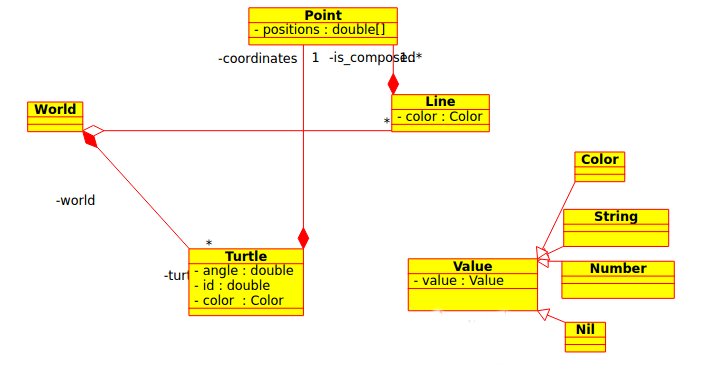
\includegraphics[scale=0.5]{doc/report/uml/v01reel.png}
\caption{\label{v0.1R} UML de la version 0.1 réalisée}
\end{figure}

Lors du seconde sprint, les types Stibbons sont les mêmes, mais leurs définitions s'est un peu complexifiées en passant par une classe \verb|SimpleValue|, pour la mise en place des mutexs. Une énumeration des types Stibbons existe, elle est utilisée avec la méthode \verb|getType()| pour pouvoir connaître le type de \verb|Value|.
Pour que l'utilisateur puisse écrire des fonctions dans le code, nous avons ajouté une classe \verb|Function|, qui stocke un arbre abstrait, contenant le code de la fonction déjà analysé.
Des mutexs ont également été ajouté dans toutes les classes pour assurer que les threads soient thread-safe (cf.~\ref{v0.2}).

\begin{figure}[h]
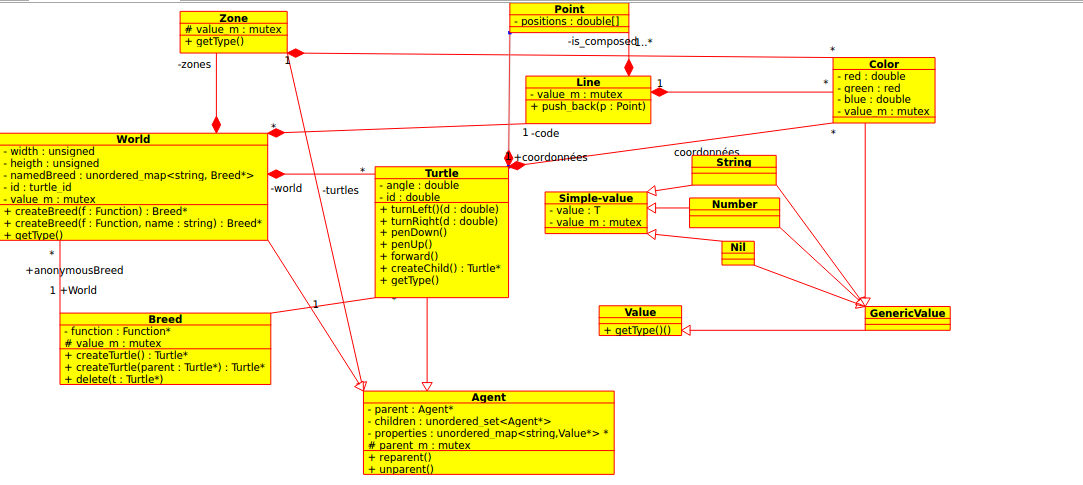
\includegraphics[scale=0.45]{doc/report/uml/v02.png}
\caption{\label{v0.2} UML version 0.2}
\end{figure}
\subsubsection{Sprints 3 et 4}
Lors du troisième sprint, nous avons ajouté une sous-classe de \verb|Function| : \verb|userFunction|, qui représentent les fonctions créées par l'utilisateur (cf. Figure~\ref{v0.3}). Nous avons également créer des fonctions standards comme \verb|ask_zone|, qui permettent de donner un ordre aux zones.
\begin{figure}[h]
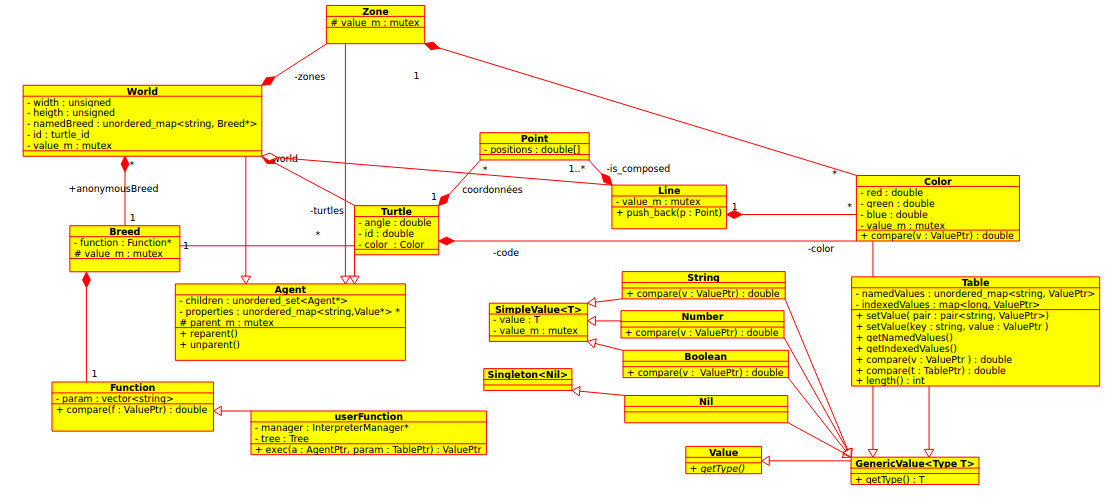
\includegraphics[scale=0.4]{doc/report/uml/v03.png}
\caption{\label{v0.3} UML version 0.3}
\end{figure}

On les différencie des instructions par leurs parenthèses derrière leur nom.
L'ajout de table fait aussi parti de ce sprint. Nous avons choisi, pour notre langage un seul type de conteneur~: les tableaux.
Nous les écrivons à la façon de php (cf. Listing~\ref{tablephp}).
\begin{lstlisting}[label=tablephp,caption=Syntaxe des tables en Stibbons]
a = 12

t = {18,red,"bla"}
v = { "bla" : "blou", "blue" : blue, a : 29 }

println(t[2])
t[2] = 32
println(t[2])
v[] = 48
println(v)

u = 5 new agent {
	while true fd 20
}
\end{lstlisting}

Nous avons mis en place des mutexs récursifs lors du quatrième sprint. Ils permettent à un thread de verrouiller plusieurs fois la même ressource qu'il a déjà verrouillée. C'est la seule différence avec le mutex normal. 

Ces mutexs permettent d'éviter des blocages dans certaines situations (fonctions récursives, etc.) .
L'UML \ref{v0.4} est l'état final du modèle car le sprint 5 n'y a apporté aucune modification.
\begin{figure}[h]
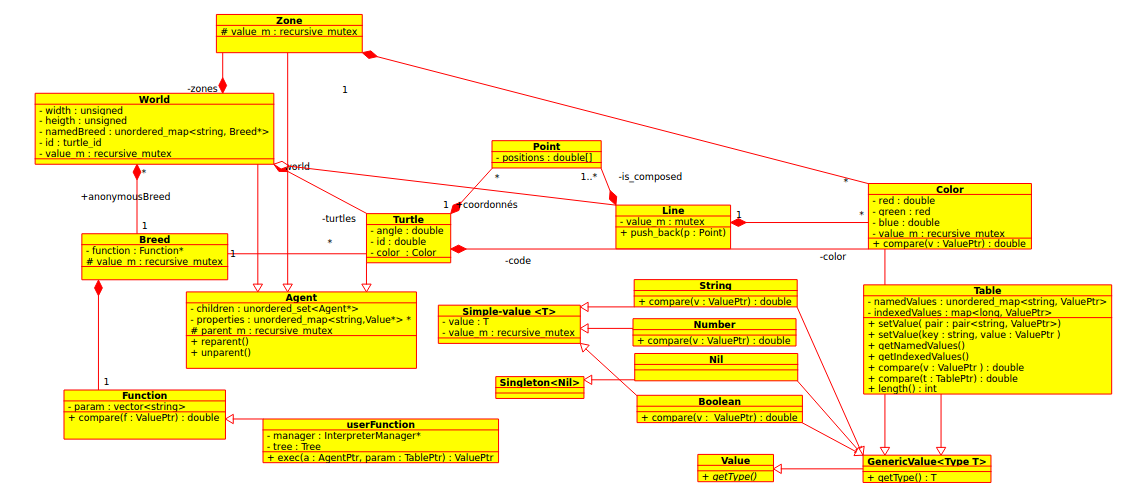
\includegraphics[scale=0.4]{doc/report/uml/v04.png}
\caption{\label{v0.4} UML version 0.4}
\end{figure}

